\documentclass[tikz,border=15pt]{standalone}
\usepackage{tikz}
\usetikzlibrary{shapes.geometric, arrows.meta, positioning, fit, backgrounds, calc, shadows, decorations.pathmorphing}

\begin{document}
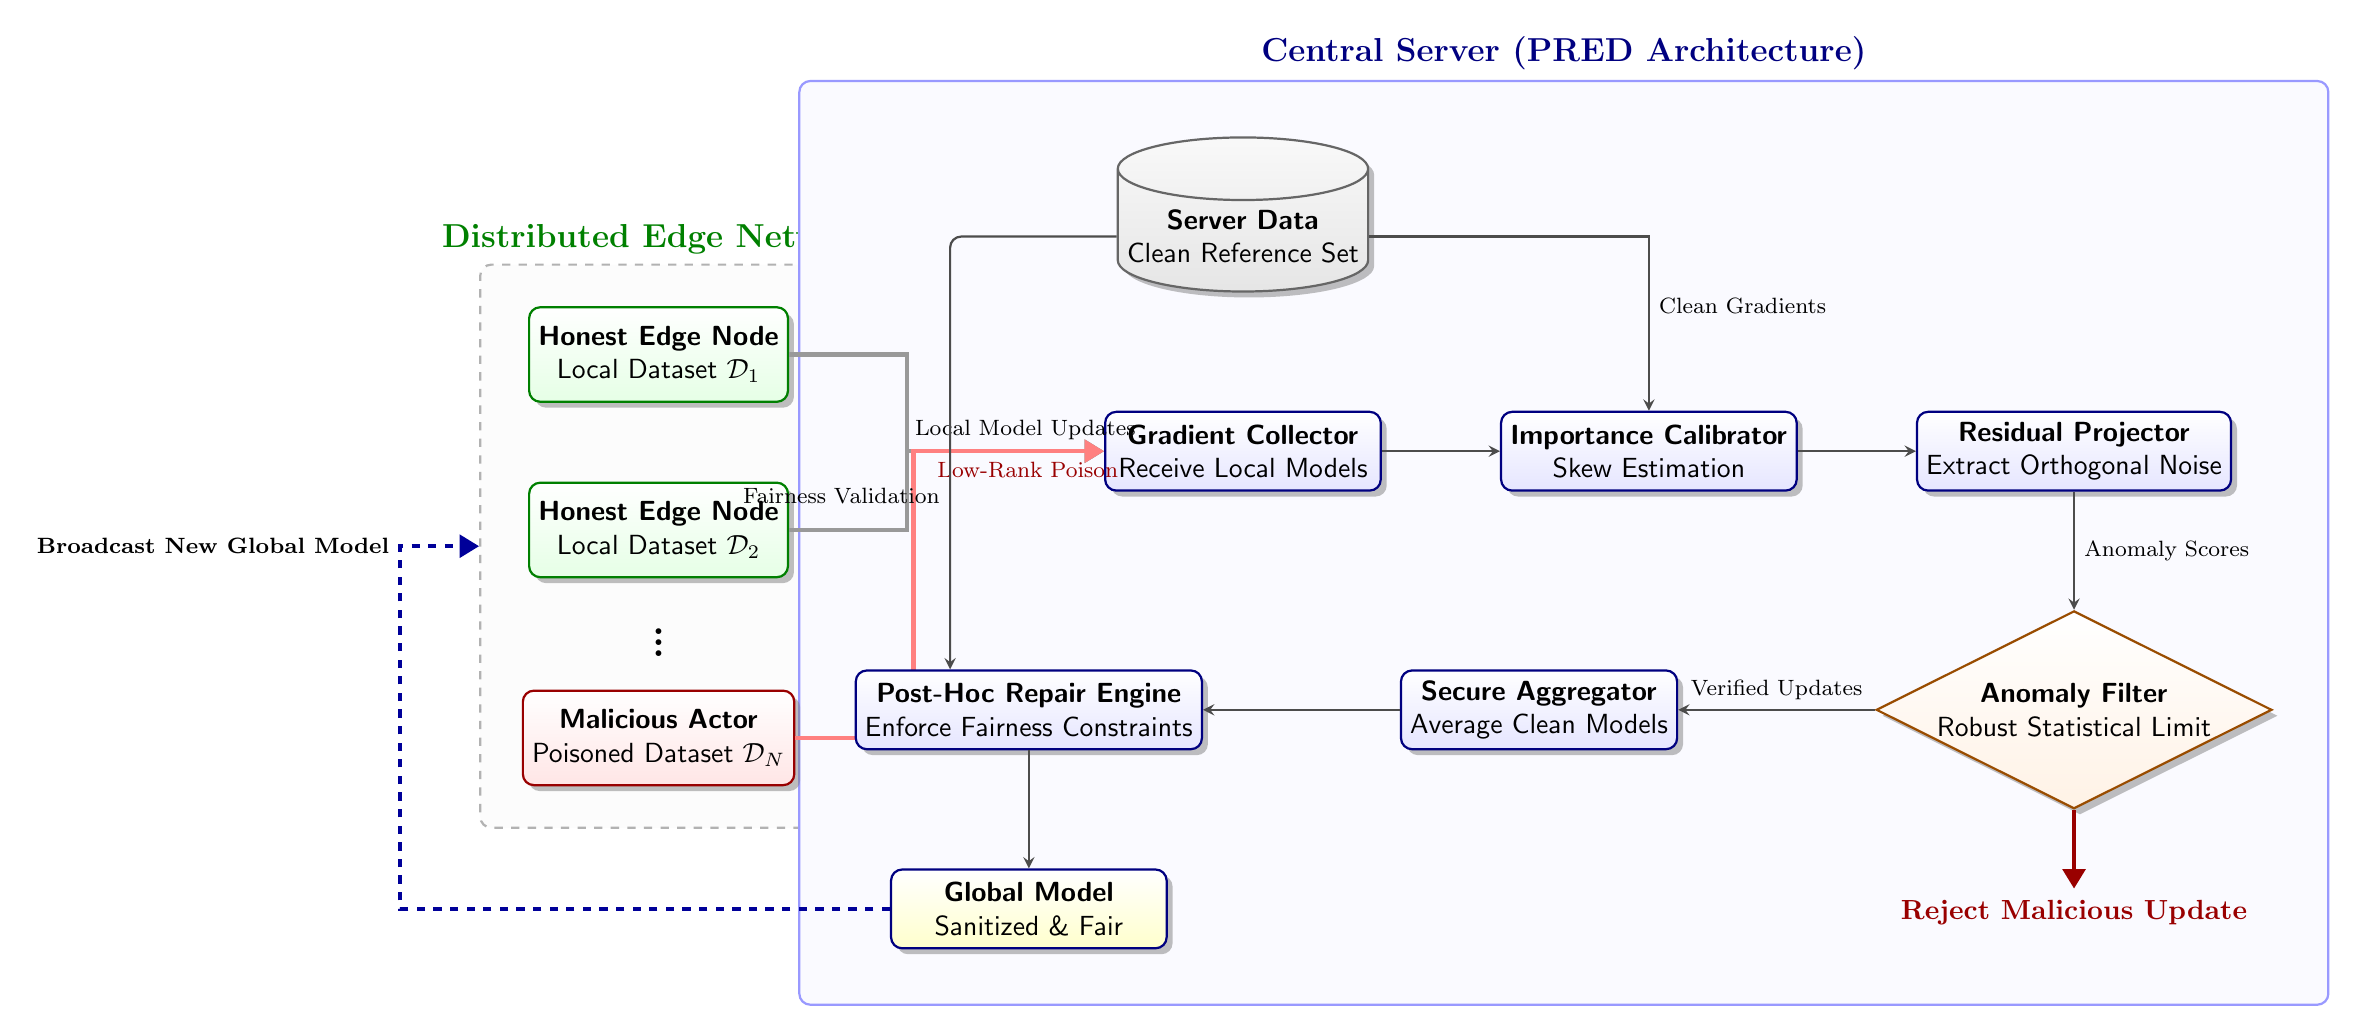
\begin{tikzpicture}[
    font=\sffamily,
    % Advanced Styles
    client_box/.style={draw=green!50!black, thick, top color=white, bottom color=green!10, rounded corners, minimum width=3cm, minimum height=1.2cm, align=center, drop shadow},
    server_module/.style={draw=blue!50!black, thick, top color=white, bottom color=blue!10, rectangle, rounded corners, minimum width=3.5cm, minimum height=1cm, align=center, drop shadow},
    decision_box/.style={draw=orange!60!black, thick, top color=white, bottom color=orange!10, diamond, aspect=2, align=center, inner sep=1pt, drop shadow},
    database/.style={draw=gray!80!black, thick, top color=gray!5, bottom color=gray!20, cylinder, shape border rotate=90, aspect=0.25, minimum height=1.5cm, minimum width=1.8cm, align=center, drop shadow},
    arrow/.style={thick, ->, >=stealth, draw=black!70},
    fat_arrow/.style={line width=1.5pt, ->, >=Triangle, draw=gray!80},
    group_box/.style={draw=gray!60, dashed, thick, inner sep=15pt, rounded corners, fill=gray!2},
    server_boundary/.style={draw=blue!40, thick, inner sep=20pt, rounded corners, fill=blue!2}
]

% ---------------- CLIENT EDGE ----------------
\node[client_box] (client1) {\textbf{Honest Edge Node}\\Local Dataset $\mathcal{D}_1$};
\node[client_box, below=1cm of client1] (client2) {\textbf{Honest Edge Node}\\Local Dataset $\mathcal{D}_2$};
\node[below=0.3cm of client2, font=\Large\bfseries] (dots) {$\vdots$};
\node[client_box, draw=red!60!black, bottom color=red!10, below=0.3cm of dots] (clientN) {\textbf{Malicious Actor}\\Poisoned Dataset $\mathcal{D}_N$};

% Group Clients
\begin{scope}[on background layer]
    \node[group_box, fit=(client1)(clientN), label={[font=\bfseries\large, text=green!50!black]above:Distributed Edge Network}] (client_env) {};
\end{scope}

% ---------------- CENTRAL SERVER ----------------
% Module 1: Collector
\node[server_module, right=4cm of client2, yshift=1cm] (collector) {\textbf{Gradient Collector}\\Receive Local Models};

% Client arrows to collector
\draw[fat_arrow] (client1.east) -- ++(1.5,0) |- (collector.west) node[pos=0.8, above, font=\footnotesize] {Local Model Updates};
\draw[fat_arrow] (client2.east) -- ++(1.5,0) |- (collector.west);
\draw[fat_arrow, draw=red!50] (clientN.east) -- ++(1.5,0) |- (collector.west) node[pos=0.8, below, font=\footnotesize, text=red!60!black] {Low-Rank Poison};

% Reference Data
\node[database, above=1.5cm of collector] (ref_data) {\textbf{Server Data}\\Clean Reference Set};

% Module 2: Profiler
\node[server_module, right=1.5cm of collector] (profiler) {\textbf{Importance Calibrator}\\Skew Estimation};
\draw[arrow] (ref_data.east) -| (profiler.north) node[pos=0.7, right, font=\footnotesize] {Clean Gradients};
\draw[arrow] (collector.east) -- (profiler.west);

% Module 3: Projector
\node[server_module, right=1.5cm of profiler] (projector) {\textbf{Residual Projector}\\Extract Orthogonal Noise};
\draw[arrow] (profiler.east) -- (projector.west);

% Module 4: Filter
\node[decision_box, below=1.5cm of projector] (filter) {\textbf{Anomaly Filter}\\Robust Statistical Limit};
\draw[arrow] (projector.south) -- (filter.north) node[midway, right, font=\footnotesize] {Anomaly Scores};

% Discard
\coordinate (discard) at ($(filter.south) - (0,1cm)$);
\draw[fat_arrow, draw=red!60!black] (filter.south) -- (discard) node[below, text=red!60!black, font=\bfseries] {Reject Malicious Update};

% Module 5: Aggregation
\node[server_module, left=2.5cm of filter] (agg) {\textbf{Secure Aggregator}\\Average Clean Models};
\draw[arrow] (filter.west) -- node[above, font=\footnotesize] {Verified Updates} (agg.east);

% Module 6: Repair
\node[server_module, left=2.5cm of agg] (repair) {\textbf{Post-Hoc Repair Engine}\\Enforce Fairness Constraints};
\draw[arrow] (agg.west) -- (repair.east);

% Connect ref data to repair
\draw[arrow, rounded corners] (ref_data.west) -| ($(repair.north) - (1cm,0)$) node[pos=0.8, left, font=\footnotesize] {Fairness Validation};

% Global Model
\node[server_module, bottom color=yellow!20, below=1.5cm of repair] (global) {\textbf{Global Model}\\Sanitized \& Fair};
\draw[arrow] (repair.south) -- (global.north);

% Group Server
\begin{scope}[on background layer]
    \node[server_boundary, fit=(ref_data)(collector)(profiler)(projector)(filter)(discard)(agg)(repair)(global), label={[font=\bfseries\large, text=blue!50!black]above:Central Server (PRED Architecture)}] (server_env) {};
\end{scope}

% ---------------- FEEDBACK ----------------
\draw[fat_arrow, dashed, draw=blue!60!black] (global.west) -| ($(client_env.west) - (1cm,0)$) |- (client_env.west) node[pos=0.25, left, font=\footnotesize\bfseries] {Broadcast New Global Model};

\end{tikzpicture}
\end{document}
